

\subsection{Determinism: Type Partitioning}

{  %% chapter slide
%  \setbeamercolor{background canvas}{bg=sectioncolor}
\begin{frame}{\Challenge{4} A Sufficient Type Partitioning}{MDTD: Maximal Disjoint Type Decomposition}
  \only<1>{Given overlapping (super)types $A_1\ldots A_n$ in an RTE}%
  \only<2>{Construct (sub) types $\typevar_1\ldots \typevar_m$}%
  \only<3>{Which are disjoint \Emph{by construction}, even if subtype relation is unknown.}%
  \only<4>{Assures that $\deriv{\typevar}{r}$ is computable.}%
  \only<5>{But transitions may be \Emph{indeterminate} and \Emph{unsatisfiable}.}%
  \begin{columns}
    \begin{column}{0.5\textwidth}
      \only<1,2>{\scalebox{0.98}{\begin{pgfpicture}{0cm}{0cm}{10cm}{6cm} % LL=0,0  UR=10,6
  \pgfcircle[stroke]{\pgfxy(3.5,3)}{3.0cm}   % A   A1
  \pgfputat{\pgfxy(3.5,5.7)}{\pgfbox[center,center]{$A_{1}$}}
  \pgfcircle[stroke]{\pgfxy(2,4)}{1.0cm}   % B    A2
  \pgfputat{\pgfxy(1.5,4.5)}{\pgfbox[center,center]{$A_{2}$}}
  \pgfcircle[stroke]{\pgfxy(3,4.2)}{1.0cm}   % C   A3
  \pgfputat{\pgfxy(3.5,4.6)}{\pgfbox[center,center]{$A_{3}$}}
  \pgfcircle[stroke]{\pgfxy(2.5,2.3)}{1.7cm}   % D A4
  \pgfputat{\pgfxy(1.2,2.7)}{\pgfbox[center,center]{$A_{4}$}}
  \pgfcircle[stroke]{\pgfxy(3.1,1.4)}{0.5cm}   % E   A5
  \pgfputat{\pgfxy(3.2,1.6)}{\pgfbox[center,center]{$A_{5}$}}
  \pgfcircle[stroke]{\pgfxy(5.5,2.0)}{0.5cm}   % F   A6
  \pgfputat{\pgfxy(5.5,2.25)}{\pgfbox[center,center]{$A_{6}$}}
  \pgfcircle[stroke]{\pgfxy(6.7,1.3)}{0.5cm}   % G   A7
  \pgfputat{\pgfxy(6.7,1.5)}{\pgfbox[center,center]{$A_{7}$}}
  \pgfcircle[stroke]{\pgfxy(3.4,1.1)}{1.0cm}   % H   A8
  \pgfputat{\pgfxy(4.0,0.8)}{\pgfbox[center,center]{$A_{8}$}}
\end{pgfpicture}
}}%
      \only<3->{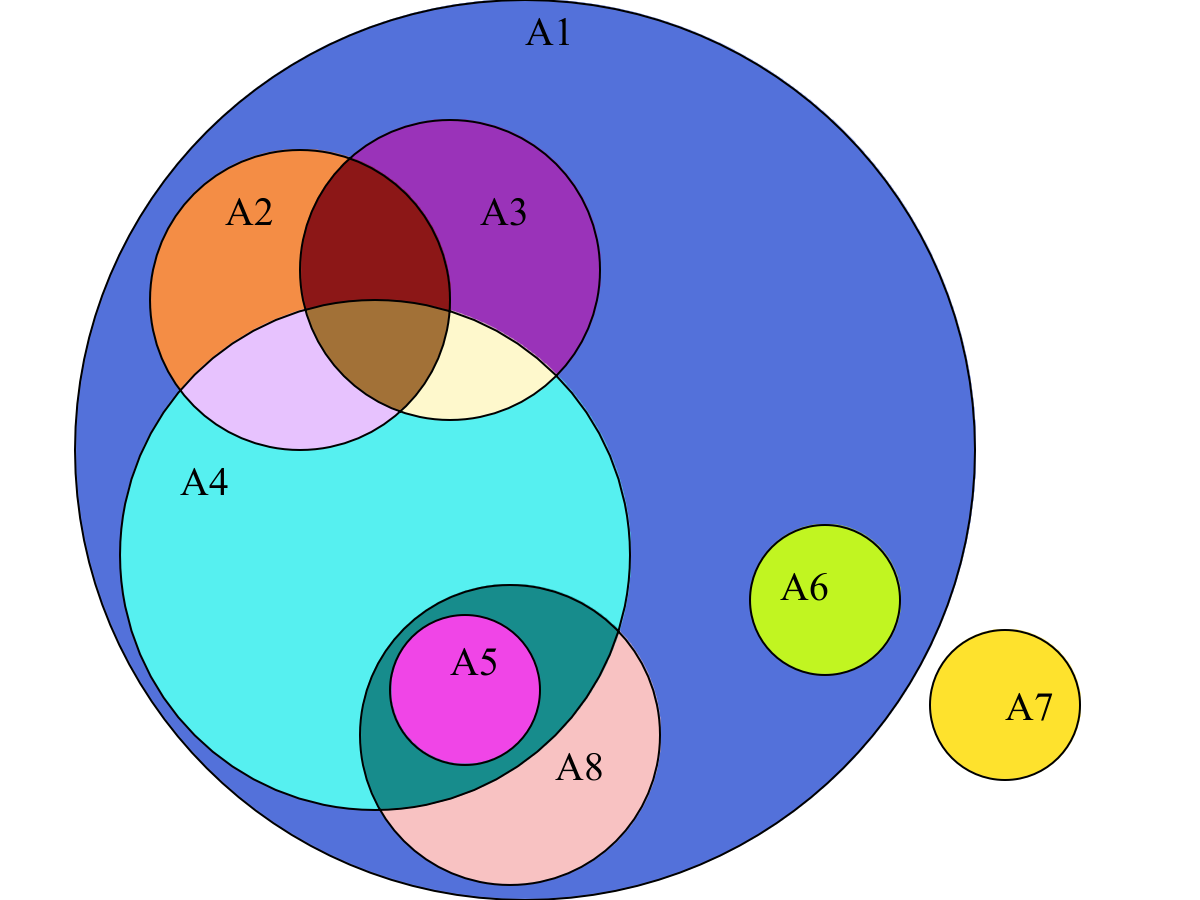
\includegraphics[scale=0.18]{venn-x1-x13.png}}%
    \end{column}%
    \begin{column}{0.5\textwidth}
      \only<2->{\scalebox{0.98}{    \begin{pgfpicture}{0cm}{0cm}{10cm}{6cm} % LL=0,0  UR=10,6
      \pgfcircle[stroke]{\pgfxy(3.5,3)}{3.0cm}   % A   A1
      \pgfputat{\pgfxy(5.5,3.7)}{\pgfbox[center,center]{$\typevar_{1}$}}
      \pgfcircle[stroke]{\pgfxy(2,4)}{1.0cm}   % B    A2
      \pgfputat{\pgfxy(1.7,4.2)}{\pgfbox[center,center]{$\typevar_{2}$}}
      \pgfcircle[stroke]{\pgfxy(3,4.2)}{1.0cm}   % C   A3
      \pgfputat{\pgfxy(2.5,4.4)}{\pgfbox[center,center]{$\typevar_{13}$}}
      \pgfputat{\pgfxy(3.5,4.1)}{\pgfbox[center,center]{$\typevar_{3}$}}
      \pgfputat{\pgfxy(2.5,3.7)}{\pgfbox[center,center]{$\typevar_{11}$}}
      \pgfputat{\pgfxy(2.0,3.4)}{\pgfbox[center,center]{$\typevar_{10}$}}
      \pgfputat{\pgfxy(3.2,3.5)}{\pgfbox[center,center]{$\typevar_{12}$}}
      \pgfcircle[stroke]{\pgfxy(2.5,2.3)}{1.7cm}   % D A4
      \pgfputat{\pgfxy(1.8,1.8)}{\pgfbox[center,center]{$\typevar_{4}$}}
      \pgfcircle[stroke]{\pgfxy(3.1,1.4)}{0.5cm}   % E   A5
      \pgfputat{\pgfxy(3.0,1.3)}{\pgfbox[center,center]{$\typevar_{5}$}}
      \pgfcircle[stroke]{\pgfxy(5.5,2.0)}{0.5cm}   % F   A6
      \pgfputat{\pgfxy(5.5,1.9)}{\pgfbox[center,center]{$\typevar_{6}$}}
      \pgfcircle[stroke]{\pgfxy(6.7,1.3)}{0.5cm}   % G   A7
      \pgfputat{\pgfxy(6.7,1.4)}{\pgfbox[center,center]{$\typevar_{7}$}}
      \pgfcircle[stroke]{\pgfxy(3.4,1.1)}{1.0cm}   % H   A8
      \pgfputat{\pgfxy(3.2,0.45)}{\pgfbox[center,center]{$\typevar_{8}$}}
      \pgfputat{\pgfxy(3.7,1.8)}{\pgfbox[center,center]{$\typevar_{9}$}}
    \end{pgfpicture}
}}%
    \end{column}%
  \end{columns}%
\end{frame}


%% \begin{frame}{Are there dire Consequences?}

%%   \begin{itemize}
%%   \item   $\{\typevar_1, \typevar_2, \ldots, \typevar_{10}\}$ mutually disjoint by construction.
%%   \item   However, some $\typevar_i$ may be unknowingly vacuous.
%%   \item   Nevertheles $\emptyset$ is disjoint with every set, including itself.
%%   \item   Thus transitions may be \Emph{indeterminate/unsatisfiable}.
%%   \item   What is the consequence transitions which are  \Emph{indeterminate} and \Emph{unsatisfiable}?
%%   \end{itemize}
%% \end{frame}

\begin{frame}{DFA with indeterminate transitions: $(int \cdot str^{*} \cdot even)^{*}$}
  \begin{columns}
    \begin{column}{0.5\textwidth}
      \begin{align*}
        p_0 &= (int \cdot str^{*} \cdot even)^{*}\\
        p_1 &= \emptyset\\
        p_2 &= \tystring^{*} \cdot \tyeven \cdot (\tyint \cdot \tystring^{*} \cdot \tyeven)^{*}\\
        p_3 &= \tystring^{*}\!\!\cdot\! \tyeven\!\cdot\! (\tyint\! \cdot\! \tystring^{*}\!\!\cdot\! \tyeven)^{*}\! \reor (\tyint\! \cdot\! \tystring^{*}\!\!\cdot\!\! \tyeven)^{*}
      \end{align*}



      \includegraphics[width=0.9\textwidth,trim={1.4cm 1.2cm 1.4cm 0.8cm},clip=true]{reclojure-2025-sink-example-2}
    \end{column}
    \begin{column}{0.5\textwidth}
      \begin{align*}
        t_1 &= \Sigma\\
        t_2 &= int  \\
        t_3 &= \compl{int}\\
        t_4 &= \textcolor{red}{str \cap even}\\
        t_5 &= \compl{str} \cap even\\
        t_6 &= str \cap \compl{even}\\
        t_7 &= (int \cap \compl{even}) \cup (str \cap \compl{even})\\
        t_8 &= \textcolor{red}{\compl{int} \cap \compl{str} \cap even}\\
        t_9 &=(int \cap even) \cup (str \cap even)\\
        t_{10} &=\compl{str} \cap \compl{even}\\
        t_{11} &=\compl{int} \cap \compl{str} \cap \compl{even}
      \end{align*}
    \end{column}
  \end{columns}
\end{frame}


%% \begin{frame}{Non-determinism by subtype}
%%   \begin{columns}[T]
%%     \begin{column}{0.4\textwidth}
%%       \centering
      
%%       \begin{align*}
%%         Int&\subseteq Number\\
%%         Int &\cap Number \neq \emptyset
%%       \end{align*}%
%%       \scalebox{0.8}{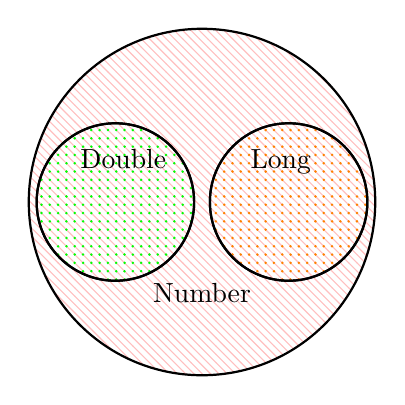
\begin{tikzpicture}[thick]
\usetikzlibrary{patterns}
  
\draw[pattern=north west lines, pattern color=pink] (0,0) circle (2.2);
\draw[pattern=dots, pattern color=orange
] (1.1,0) circle (1.0);
\draw[pattern=dots, pattern color=green
] (-1.1,0) circle (1.0);
\draw (1,0.8)     node [text=black,below] {Long};
\draw (-1,0.8)     node [text=black,below] {Double};
\draw (1.1,0) circle (1)  ;
\draw (-1.1,0) circle (1)  ;
\draw (0.0,-0.9) node [text=black,below] {Number};
\end{tikzpicture}

}%
%%     \end{column}%
%%     \begin{column}{0.6\textwidth}
%%       \only<1>{\scalebox{0.9}{\documentclass{standalone}
  \usepackage{tikz}
  \usetikzlibrary{arrows.meta, automata, bending, positioning, shapes.misc}
  \tikzstyle{automaton}=[shorten >=1pt, >={Stealth[bend,round]}, initial text=]

\begin{document}
\begin{tikzpicture}[automaton, auto, thick]
  \node[state,initial,rounded rectangle] (0) {$0$};
  \node[state,rounded rectangle] (1) [right=10mm of 0] {$1$};
  \node[state,rounded rectangle] (2) [above right=7mm and 20mm of 1] {$2$};
  \node[state,rounded rectangle] (4) [below right=7mm and 20mm of 1] {$4$};
  \path[->] (0) edge node {$Long$} (1);
  \path[->] (1) edge[color=nondeterministic, line width=3pt, bend left=15]  node[pos=.8] {$Long$} (2);
  \path[->] (1) edge[color=nondeterministic, line width=3pt, bend right=15] node[swap] {$Number$} (4);
\end{tikzpicture}
\end{document}
}}%
%%       \only<2>{\scalebox{0.8}{\documentclass{standalone}
  \usepackage{tikz}
  \usetikzlibrary{arrows.meta, automata, bending, positioning, shapes.misc}
  \tikzstyle{automaton}=[shorten >=1pt, >={Stealth[bend,round]}, initial text=]

\begin{document}
\begin{tikzpicture}[automaton, auto, thick]
  \node[state,initial,rounded rectangle] (0) {$0$};
  \node[state,rounded rectangle] (1) [right=10mm of 0] {$1$};
  \node[state,rounded rectangle] (2) [above right=28mm and 30mm of 1] {$2$};
  \node[state,rounded rectangle] (3) [above right=7mm and 30mm of 1] {$3$};
  \node[state,rounded rectangle] (4) [below right=7mm and 30mm of 1] {$4$};
  \node[state,rounded rectangle] (5) [below right=28mm and 30mm of 1] {$5$};
  \path[->] (0) edge node {$Int$} (1);
  \path[->] (1) edge[color=deterministic, line width=3pt, bend left=15]  node[pos=.8] {$Int \cap Number$} (2);
  \path[->] (1) edge[color=deterministic, line width=3pt, bend right=15] node[swap] {$Int ~\cap ~!Number$} (3);
  \path[->] (1) edge[color=deterministic, line width=3pt, bend left=15]  node[pos=.8] {$!Int \cap Number$} (4);
  \path[->] (1) edge[color=deterministic, line width=3pt, bend right=15] node[swap] {$!Int~ \cap ~!Number$} (5);
\end{tikzpicture}
\end{document}
}}%
%%     \end{column}
%%   \end{columns}
%% \end{frame}


%% \begin{frame}{Non-determinism by \code{(satisfies f)}}
%%   \begin{columns}[T]
%%     \begin{column}{0.35\textwidth}
%%       \centering
%%       \begin{align*}
%%         Odd&\subseteq Int &\text{unknown}\\
%%         Odd&~\cap~ !Int = \emptyset &\text{unknown}
%%       \end{align*}
%%       \scalebox{1.0}{\begin{tikzpicture}[thick]
\usetikzlibrary{patterns}
  
\draw[pattern=dots, pattern color=orange
] (0.1,0) circle (1.5);
\draw[pattern=north east lines, pattern color=gold
] (0.1,0) circle (0.6);

\draw (0,0.3)     node [text=black,below] {Odd};
\draw (0,1.2)     node [text=black,below] {Int};
\end{tikzpicture}

}%
%%     \end{column}%
%%     \begin{column}{0.7\textwidth}
%%       \only<1>{\scalebox{0.9}{\documentclass{standalone}
  \usepackage{tikz}
  \usetikzlibrary{arrows.meta, automata, bending, positioning, shapes.misc}
  \tikzstyle{automaton}=[shorten >=1pt, >={Stealth[bend,round]}, initial text=]

\begin{document}
\begin{tikzpicture}[automaton, auto, thick]
  \node[state,initial,rounded rectangle] (0) {$0$};
  \node[state,rounded rectangle] (1) [right=10mm of 0] {$1$};
  \node[state,rounded rectangle] (2) [above right=20mm and 30mm of 1] {$2$};
  \node[state,rounded rectangle] (4) [below right=20mm and 30mm of 1] {$4$};
  \path[->] (0) edge node {$Long$} (1);
  \path[->] (1) edge[color=nondeterministic, line width=3pt, bend left=15]  node[pos=.8] {$Long$} (2);
  \path[->] (1) edge[color=nondeterministic, line width=3pt, bend right=15] node[swap] {$Odd$} (4);
\end{tikzpicture}
\end{document}
}}%
%%       \only<2>{\scalebox{0.8}{\documentclass{standalone}
  \usepackage{tikz}
  \usetikzlibrary{arrows.meta, automata, bending, positioning, shapes.misc}
  \tikzstyle{automaton}=[shorten >=1pt, >={Stealth[bend,round]}, initial text=]

\begin{document}
\begin{tikzpicture}[automaton, auto, thick]
  \node[state,initial,rounded rectangle] (0) {$0$};
  \node[state,rounded rectangle] (1) [right=10mm of 0] {$1$};
  \node[state,rounded rectangle] (2) [below right=25mm and 40mm of 1] {$2$};
  \node[state,rounded rectangle] (3) [above right=25mm and 40mm of 1] {$3$};
  \node[state,rounded rectangle] (4) [above right=5mm and 55mm of 1] {$4$};
  \node[state,rounded rectangle] (5) [below right=5mm and 55mm of 1] {$5$};
  \path[->] (0) edge node {$Int$} (1);
  \path[->] (1) edge[color=deterministic, line width=3pt, bend right=15]  node[pos=.7,swap] {$Int \cap Odd$} (2);
  \path[->] (1) edge[color=deterministic, line width=3pt, bend left=15]  node[pos=.8] {$Int~ \cap ~!Odd $} (3);
  \path[->] (1) edge[color=deterministic, line width=3pt, bend left=15]  node[pos=.5,swap] {$!Int \cap Odd$} (4);
  \path[->] (1) edge[color=deterministic, line width=3pt, bend right=15]  node[pos=.5] {$!Int~ \cap~ !Odd$} (5);
\end{tikzpicture}
\end{document}
}}%
%%     \end{column}
%%   \end{columns}
%% \end{frame}



% Double and Odd + Double and Even


% classes A and B
% if A and B are final, then they are disjoint
% if A and B are abstract, there MIGHT be a common subclass
% if A and B are in a subtype relation, then either A &! B or B & !A is empty




%% \begin{frame}{Unsatisfiable Transitions}

%%   \scalebox{0.8}{\documentclass{standalone}
  \usepackage{tikz}
  \usetikzlibrary{arrows.meta, automata, bending, positioning, shapes.misc}
  \tikzstyle{automaton}=[shorten >=1pt, >={Stealth[bend,round]}, initial text=]
  \tikzstyle{accepting}=[double]

\begin{document}
\begin{tikzpicture}[automaton, auto, thick]
  \node[state,color=green,text=black,initial,rounded rectangle] (0) {$0$};
  \node[state,color=red,text=black,rounded rectangle] (1) [right=35mm of 0] {$1$};
  \node[state,color=red,text=black,accepting,rounded rectangle] (2) [above right=7mm and 30mm of 1] {$2$};
  \node[state,color=red,text=black,accepting,rounded rectangle] (3) [below right=7mm and 30mm of 1] {$3$};
  \path[->] (0) edge[color=unsatisfiable, dotted, line width=3pt] node {$Int\cap\overline{Number}$} (1);
  \path[->] (1) edge[dashed, bend left=15, line width=2pt]  node[pos=.8] {Int} (2);
  \path[->] (1) edge[dashed, bend right=15, line width=2pt] node[swap] {String} (3);
  \path[->] (2) edge[dashed, bend left=15, line width=2pt]  node {Int} (1);
  \path[->] (2) edge[dashed, loop above, line width=2pt]    node {Int} (2);
  \path[->] (3) edge[dashed, bend right=15, line width=2pt] node[swap] {Int} (1);
  \path[->] (3) edge[dashed, loop below, line width=2pt]    node {String} (3);
\end{tikzpicture}
\end{document}
}
%%   \begin{itemize}
%%   \item If we (compile-time) determine a type is empty, then the transition is \Emph{unsatisfiable}.
%%   \item Thus we \Emph{can eliminate} the transition and unreachable states.

%%   \end{itemize}
%% \end{frame}


%% \begin{frame}{Indeterminate Transitions}

%%   \begin{tabular}{cc}
%%     \scalebox{0.7}{\documentclass{standalone}
  \usepackage{tikz}
  \usetikzlibrary{arrows.meta, automata, bending, positioning, shapes.misc}
  \tikzstyle{automaton}=[shorten >=1pt, >={Stealth[bend,round]}, initial text=]
  \tikzstyle{accepting}=[double]

\begin{document}
\begin{tikzpicture}[automaton, auto, thick]
  \node[state,color=green,text=black,initial,rounded rectangle] (0) {$0$};
  \node[state,color=red,text=black,rounded rectangle] (1) [right=35mm of 0] {$1$};
  \node[state,color=red,text=black,accepting,rounded rectangle] (2) [above right=7mm and 30mm of 1] {$2$};
  \node[state,color=red,text=black,accepting,rounded rectangle] (3) [below right=7mm and 30mm of 1] {$3$};
  \path[->] (0) edge[color=indeterminate, dotted, line width=3pt] node {$Str \cap Odd$} (1);
  \path[->] (1) edge[bend left=15]  node[pos=.8] {Int} (2);
  \path[->] (1) edge[bend right=15] node[swap] {String} (3);
  \path[->] (2) edge[bend left=15]  node {Int} (1);
  \path[->] (2) edge[loop above]    node {Int} (2);
  \path[->] (3) edge[bend right=15] node[swap] {Int} (1);
  \path[->] (3) edge[loop below]    node {String} (3);
\end{tikzpicture}
\end{document}
}&\scalebox{0.7}{\documentclass{standalone}
  \usepackage{tikz}
  \usetikzlibrary{arrows.meta, automata, bending, positioning, shapes.misc}
  \tikzstyle{automaton}=[shorten >=1pt, >={Stealth[bend,round]}, initial text=]
  \tikzstyle{accepting}=[double]

\begin{document}
\begin{tikzpicture}[automaton, auto, thick]
  \node[state,color=green,text=black,initial,rounded rectangle] (0) {$0$};
  \node[state,color=green,text=black,rounded rectangle] (1) [right=35mm of 0] {$1$};
  \node[state,color=green,text=black,accepting,rounded rectangle] (2) [above right=7mm and 30mm of 1] {$2$};
  \node[state,color=green,text=black,accepting,rounded rectangle] (3) [below right=7mm and 30mm of 1] {$3$};
  \path[->] (0) edge[color=indeterminate, dotted, line width=3pt] node {$Int \cap Odd$} (1);
  \path[->] (1) edge[bend left=15]  node[pos=.8] {Int} (2);
  \path[->] (1) edge[bend right=15] node[swap] {String} (3);
  \path[->] (2) edge[bend left=15]  node {Int} (1);
  \path[->] (2) edge[loop above]    node {Int} (2);
  \path[->] (3) edge[bend right=15] node[swap] {Int} (1);
  \path[->] (3) edge[loop below]    node {String} (3);
\end{tikzpicture}
\end{document}
}\\
%%     Indeterminate, \textcolor{red}{Unsatisfiable} & Indeterminate, \textcolor{greeny}{Satisfiable}
%%   \end{tabular}
%%   \only<1>{%
%%   \begin{itemize}
%%   \item   If we cannot determine a type is empty, the transition may
%%     \Emph{still be unsatisfiable}. 
%%   \item  However, we \Emph{cannot eliminate}    the transition and unreachable states.
%%   \end{itemize}
%%   }%
%%   \only<2>{%
%%   \begin{itemize}
%%     \item We \Emph{can always} (run-time) determine \Emph{type membership}.
%%     \item DFAs with indeterminate transitions \Emph{correctly}
%%       match sequences in $O(n)$.
%%   \end{itemize}
%%   }
%% \end{frame}


